%%%%%%%%%%%%%%%%%%%%%%%%%%%%%%%%%%%%%%%%%
% Sullivan Business Report
% LaTeX Template
% Version 1.0 (May 5, 2022)
%
% This template originates from:
% https://www.LaTeXTemplates.com
%
% Author:
% Vel (vel@latextemplates.com)
%
% License:
% CC BY-NC-SA 4.0 (https://creativecommons.org/licenses/by-nc-sa/4.0/)
%
%%%%%%%%%%%%%%%%%%%%%%%%%%%%%%%%%%%%%%%%%

%----------------------------------------------------------------------------------------
%	CLASS, PACKAGES AND OTHER DOCUMENT CONFIGURATIONS
%----------------------------------------------------------------------------------------

\documentclass[
	a4paper, % Paper size, use either a4paper or letterpaper
	12pt, % Default font size, the template is designed to look good at 12pt so it's best not to change this
	%unnumberedsections, % Uncomment for no section numbering
]{include/CSSullivanBusinessReport}

\addbibresource{include/sample.bib} % BibLaTeX bibliography file

%-----------------------------------------------------------------------
%	REPORT INFORMATION
%-----------------------------------------------------------------------
\reporttitle{} % The report title to appear on the title page and page headers, do not create manual new lines here as this will carry over to page headers

\reportsubtitle{A professional layout featuring a large margin\\ and examples of typical business report content} % Report subtitle, include new lines if needed

\reportauthors{Template created by:\\\smallskip Vel (vel@latextemplates.com)} % Report authors/group/department, include new lines if needed

\reportdate{\today} % Report date, include new lines for additional information if needed

\rightheadercontent{
\includegraphics[width=3cm]{./include/creodocs_logo.pdf}} % The content in the right header, you may want to add your own company logo or use your company/department name or leave this command empty for no right header content

\def\tightlist{}
%------------------------------------------------------------------------

\begin{document}

%------------------------------------------------------------------------
%	TITLE PAGE
%------------------------------------------------------------------------
\thispagestyle{empty} % Suppress headers and footers on this page

\begin{fullwidth} % Use the whole page width
	\vspace*{-0.075\textheight} % Pull logo into the top margin
	
	\hfill
\includegraphics[width=5cm]{./include/creodocs_logo.pdf} % Company logo

	\vspace{0.15\textheight} % Vertical whitespace

	\parbox{0.9\fulltextwidth}{\fontsize{50pt}{52pt}\selectfont\raggedright\textbf{\reporttitle}\par} % Report title, intentionally at less than full width for nice wrapping. Adjust the width of the \parbox and the font size as needed for your title to look good.
	
	\vspace{0.03\textheight} % Vertical whitespace
	
	{\LARGE\textit{\textbf{\reportsubtitle}}\par} % Subtitle
	
	\vfill % Vertical whitespace
	
	{\Large\reportauthors\par} % Report authors, group or department
	
	\vfill\vfill\vfill % Vertical whitespace
	
	{\large\reportdate\par} % Report date
\end{fullwidth}

\newpage

%----------------------------------------------------------------------------------------
%	DISCLAIMER/COPYRIGHT PAGE
%----------------------------------------------------------------------------------------
\thispagestyle{empty} % Suppress headers and footers on this page

\begin{twothirdswidth} % Content in this environment to be at two-thirds of the whole page width
	\footnotesize % Reduce font size
	
	\subsection*{Disclaimer}

	Lorem ipsum dolor sit amet, consectetur adipiscing elit. Praesent porttitor arcu luctus, imperdiet urna iaculis, mattis eros. Pellentesque iaculis odio vel nisl ullamcorper, nec faucibus ipsum molestie. Sed dictum nisl non aliquet porttitor. Etiam vulputate arcu dignissim, finibus sem et, viverra nisl. Aenean luctus congue massa, ut laoreet metus ornare in. Nunc fermentum nisi imperdiet lectus tincidunt vestibulum at ac elit.
	
	\subsection*{Copyright}
	
	\textcopyright~[Year] [Company] 
	
	Copyright notice text\ldots In hac habitasse platea dictumst. Curabitur mattis elit sit amet justo luctus vestibulum. In hac habitasse platea dictumst. Pellentesque lobortis justo enim, a condimentum massa tempor eu. Ut quis nulla a quam pretium eleifend nec eu nisl. Nam cursus porttitor eros, sed luctus ligula convallis quis.
	
	\subsection*{Contact}
	
	Address Line 1\\
	Address Line 2\\
	Address Line 3
	
	Business Number 123456
	
	Contact: name@company.com
	
	\vfill % Push the following down to the bottom of the page
	
	\subsubsection*{Changelog}
	
	\scriptsize % Reduce font size further
	
	\begin{tabular}{@{} L{0.05\linewidth} L{0.15\linewidth} L{0.6\linewidth} @{}} % Column widths specified here, change as needed for your content
		\toprule
		v1.0 & 20XX-02-05 & Lorem ipsum dolor sit amet, consectetur adipiscing elit. Praesent porttitor arcu luctus, imperdiet urna iaculis, mattis eros.\\
		v1.1 & 20XX-02-27 & Pellentesque iaculis odio vel nisl ullamcorper, nec faucibus ipsum molestie.\\
		v1.2 & 20XX-03-15 & Sed dictum nisl non aliquet porttitor.\\
		\bottomrule
	\end{tabular}
\end{twothirdswidth}

\newpage

%----------------------------------------------------------------------------------------
%	TABLE OF CONTENTS
%----------------------------------------------------------------------------------------
\begin{twothirdswidth} % Content in this environment to be at two-thirds of the whole page width
	\tableofcontents % Output the table of contents, automatically generated from the section commands used in the document
\end{twothirdswidth}

\newpage

%----------------------------------------------------------------------------------------
%	SECTIONS
%----------------------------------------------------------------------------------------

\newpage

\section{Dominio de Aplicaciones
SG}\label{sec:dominio-de-aplicaciones-sg}

\subsection{Análisis de Entorno Sistemas de Información
SG}\label{sec:anuxe1lisis-de-entorno-sistemas-de-informaciuxf3n-sg}

\begin{quote}
Arquitectura Empresarial SG. Ingenium. 2025 Dominio de Sistemas y
Aplicaciones de Software. Sistemas de información del análisis de
entorno.
\end{quote}

La consultoría de arquitectura empresarial busca fortalecer la
alineación de estrategias, procesos y tecnologías, así como impulsar la
transformación digital y una gestión pública más eficiente. Esta
iniciativa se enmarca en la necesidad de mejorar la satisfacción de los
grupos de interés internos y externos.

Las relaciones entre los sistemas de información (Anexo Técnico) y el
contexto del Análisis de Entorno (Resumen Ejecutivo FASE I.pdf) son las
siguientes:

\begin{itemize}
\tightlist
\item
  Sistemas de gestión administrativa y financiera (ADMON, Administrativo
  y Financiero, SIGA, SAT Web, GLPI):

  \begin{itemize}
  \tightlist
  \item
    Estos sistemas son cruciales para la ``Gestión financiera'',
    ``Gestión de servicios administrativos y tecnológicos'' y ``Gestión
    de recursos físicos''.
  \item
    Relación con objetivos: El ``Resumen Ejecutivo FASE I.pdf'' aborda
    la necesidad de una gestión pública más eficiente y transparente, la
    optimización de recursos y la rendición de cuentas. Estos sistemas
    son habilitadores directos de dichas metas.
  \item
    Relación con problemas: El documento también señala desafíos en el
    ``Entorno Económico'' como el déficit fiscal y la necesidad de
    eficiencia en la inversión pública. Los sistemas administrativos y
    financieros son fundamentales para una planificación financiera
    adecuada y una gestión fiscal sostenible.
  \item
    Relación con oportunidades: La recomendación de ``simplificación
    administrativa y coordinación intersectorial'' implica la mejora de
    estos sistemas para reducir duplicidades y estandarizar prácticas,
    lo que contribuye a una ``arquitectura institucional más coherente y
    eficiente''.
  \end{itemize}
\item
  Sistemas de interacción ciudadana y transparencia (Bogotá Te Escucha,
  Datos para la Transparencia (SATI), EMLAZE):

  \begin{itemize}
  \tightlist
  \item
    Estos sistemas soportan directamente el proceso de ``Gobierno
    abierto y relacionamiento con la ciudadanía''.
  \item
    Objetivos: El ``Resumen Ejecutivo FASE I.pdf'' destaca el objetivo
    estratégico ``Bogotá confía en su gobierno'', que busca ofrecer
    ``servicios amables, ágiles y oportunos''. Bogotá Te Escucha es el
    sistema distrital clave para la gestión de peticiones ciudadanas y
    la evaluación de la calidad de las respuestas.
  \item
    Problemas: Se reconoce que, si bien hay avances en la atención
    institucional, persisten desafíos en la ``eficiencia operativa,
    tiempos de respuesta y digitalización de servicios''. Estos sistemas
    son vitales para abordar estas brechas mediante la digitalización de
    servicios públicos y la automatización de trámites.
  \item
    Oportunidad: ``Datos para la Transparencia (SATI)'' es clave para la
    política de ``Transparencia, acceso a la información pública y lucha
    contra la corrupción''. La estandarización de procesos y sistemas de
    información a través de estos sistemas fortalece la confianza
    ciudadana.
  \end{itemize}
\item
  Sistemas de fortalecimiento de capacidades y conocimiento (Bogotá
  Aprende TIC, DARUMA, GLOBO, SUDIVC, HUMANAPP, SIAB (El COFRE), KOHA,
  SIVIC, Data Warehouse AVANTI, Gestión Académica):
\end{itemize}

\paragraph{Relación con Objetivos}\label{sec:relaciuxf3n-con-objetivos}

\begin{itemize}
\tightlist
\item
  Bogotá Aprende TIC y Gestión Académica abordan la necesidad de
  ``alfabetización digital'' y la escasez de talento humano
  especializado en tecnologías emergentes, como se menciona en el
  ``Entorno Tecnológico''.
\item
  DARUMA es el aplicativo donde se gestionan las fichas técnicas de
  productos y servicios y los riesgos estratégicos. Esto se alinea con
  la necesidad de una ``Gestión del riesgo'' efectiva y el
  ``Fortalecimiento de la Gestión Pública'' para la toma de decisiones
  basada en evidencia.
\item
  HUMANAPP es fundamental para la ``Gestión del talento humano''. El
  ``Resumen Ejecutivo FASE I.pdf'' subraya la importancia de la
  ``profesionalización del servicio público'' y el ``fortalecimiento de
  capacidades'' de los servidores públicos.
\item
  SIAB (El COFRE), KOHA, Data Warehouse AVANTI son cruciales para la
  ``Gestión del conocimiento'' y la ``Gestión documental y soporte
  archivístico''. El documento enfatiza el ``fortalecimiento de las
  capacidades de generación, análisis y uso estratégico de información''
  y la necesidad de ``sistemas integrados de datos'' para la toma de
  decisiones basada en evidencia. Data Warehouse AVANTI, en particular,
  facilita el análisis descriptivo, predictivo y prospectivo de los
  resultados de la gestión.
\item
  SUDIVC y SIVIC apoyan los procesos de ``Paz, víctimas y
  reconciliación'' y ``Fortalecimiento de la Gestión Pública'',
  abordando las ``profundas desigualdades que afectan de manera
  desproporcionada a poblaciones vulnerables'' y contribuyendo a que
  Bogotá sea un ``territorio de paz y reconciliación''.
\end{itemize}

\paragraph{Relación con
Oportunidades}\label{sec:relaciuxf3n-con-oportunidades}

\begin{itemize}
\tightlist
\item
  GitLab, siendo una plataforma de desarrollo y colaboración, está
  vinculada con la ``Gestión de alianzas e internacionalización de
  Bogotá''.
\item
  El ``Resumen Ejecutivo FASE I.pdf'' menciona la consolidación de
  Bogotá como una ciudad con ``vocación internacional, atrayendo a
  profesionales, diplomáticos, académicos y organizaciones'' y la
  necesidad de ``fortalecer la arquitectura Internacional del
  Distrito''. GitLab puede ser una herramienta para facilitar la
  colaboración en proyectos y la gestión de información en el marco de
  estas alianzas.
\item
  También se alinea con la necesidad de ``integración entre plataformas
  digitales institucionales'' y la adopción de nuevas tecnologías para
  la ``transformación digital''.
\end{itemize}

\begin{figure}
\centering
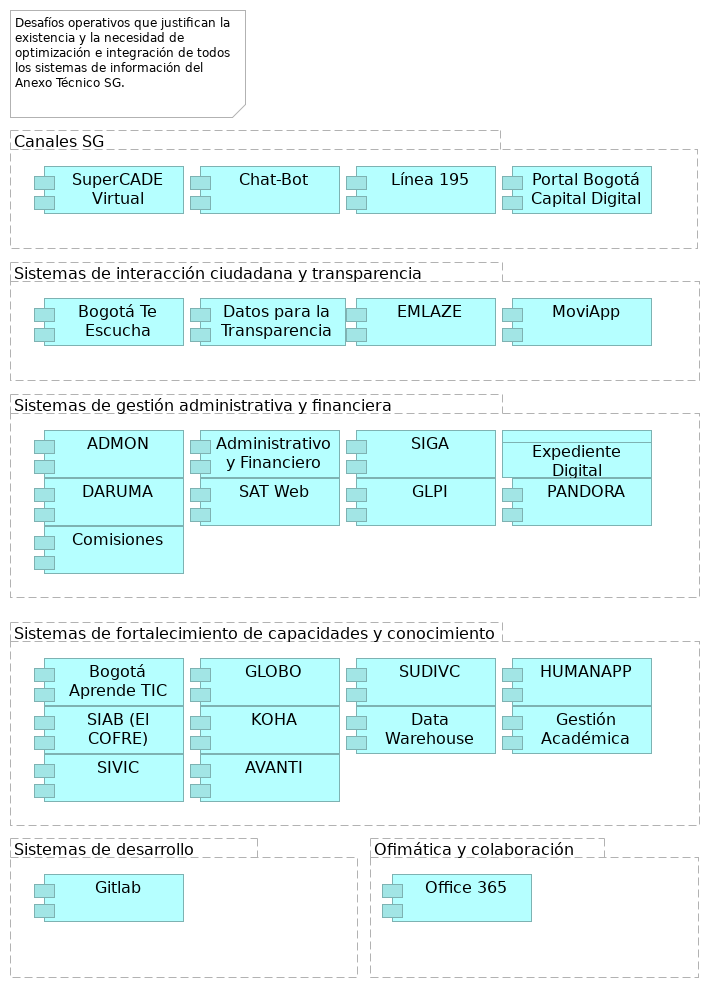
\includegraphics{images/06.2n2.SIdelAnalisisdeEntorno.png}
\caption{06.2n2. SI del Analisis de Entorno. \emph{Fuente: Propuesta
servicios de ingeniería y evaluación de arquitectura Arquitectura de
Aplicaciones Secretaria de la Alcaldía de Bogotá
(2025)}}\label{fig:id-097745511d984e7eaf02b5ad5a93e7a8}
\end{figure}

\subsubsection{Elementos del Modelo}\label{sec:elementos-del-modelo}

\begin{longtable}[]{@{}
  >{\raggedright\arraybackslash}p{(\columnwidth - 4\tabcolsep) * \real{0.3000}}
  >{\raggedright\arraybackslash}p{(\columnwidth - 4\tabcolsep) * \real{0.2000}}
  >{\raggedright\arraybackslash}p{(\columnwidth - 4\tabcolsep) * \real{0.5000}}@{}}
\caption{\label{tbl:tblelement-06.2n2.SIdelAnalisisdeEntorno-id}Elementos
de la vista.}\tabularnewline
\toprule\noalign{}
\begin{minipage}[b]{\linewidth}\raggedright
Nombre
\end{minipage} & \begin{minipage}[b]{\linewidth}\raggedright
Tipo
\end{minipage} & \begin{minipage}[b]{\linewidth}\raggedright
Documentación
\end{minipage} \\
\midrule\noalign{}
\endfirsthead
\toprule\noalign{}
\begin{minipage}[b]{\linewidth}\raggedright
Nombre
\end{minipage} & \begin{minipage}[b]{\linewidth}\raggedright
Tipo
\end{minipage} & \begin{minipage}[b]{\linewidth}\raggedright
Documentación
\end{minipage} \\
\midrule\noalign{}
\endhead
\bottomrule\noalign{}
\endlastfoot
Canales Alcaldía & Grouping & \\
SuperCADE Virtual & Application Component & Red de canales presenciales
de atención a ciudadanía. \\
& & \\
Chat-Bot & Application Component & Canal web de atención a
ciudadanía. \\
& & \\
Línea 195 & Application Component & Canal telefónico de atención a
ciudadanía. \\
& & \\
Portal Bogotá Capital Digital & Application Component & Plataforma de
Trámites en línea. Portal Integrador de trámites y servicios ofrecidos a
la ciudadanía. Componente de aplicación que permite la realización de
trámites digitales. \\
& & \\
Sistema de Participación Ciudadana & Application Component & Componente
de aplicación para facilitar la interacción y el acercamiento
(realimentación) de los ciudadanos. \\
& & \\
Sistemas de interacción ciudadana y transparencia & Grouping & \\
Bogotá Te Escucha & Application Component & Es fundamental para el
proceso de Gobierno abierto y relacionamiento con la ciudadanía. También
se menciona como el Sistema Distrital para la Gestión de Peticiones
Ciudadanas, a través del cual se evalúa la calidad de las respuestas
emitidas a la ciudadanía. \\
& & \\
Datos para Transparencia (SATI) & Application Component & Plataforma que
facilita el acceso público a datos e información gubernamental. Soporta
el proceso de Gobierno abierto y relacionamiento con la ciudadanía. \\
& & \\
EMLAZE & Application Component & Utilizado en los procesos de Gobierno
abierto y relacionamiento con la ciudadanía, y Fortalecimiento de la
Gestión Pública. \\
& & \\
MoviApp & Application Component & Canal movil de atención a ciudadanía.
Sesión levantamiento no. 2. \\
& & \\
Sistemas de gestión administrativa y financiera & Grouping & \\
ADMON & Application Component & Se relaciona con la gestión financiera,
gestión de servicios administrativos y tecnológicos, y gestión de
recursos físicos. \\
& & \\
Administrativo y Financiero & Application Component & Soporta la gestión
financiera, gestión de servicios administrativos y tecnológicos, y
gestión de recursos físicos. \\
& & \\
SIGA & Application Component & Interviene en la gestión de contratación,
gestión financiera, gestión de servicios administrativos y tecnológicos,
y gestión de recursos físicos. \\
& & \\
Sistema Gestión Documental & Application Component & Componente de
aplicación para la gestión electrónica de documentos. \\
& & \\
DARUMA & Application Component & Se utiliza en el proceso de
Fortalecimiento de la Gestión Pública. También es el aplicativo donde se
encuentran definidas las fichas técnicas de productos y servicios de la
Secretaría General y se gestionan los riesgos estratégicos. \\
& & \\
SAT Web & Application Component & Relacionado con la gestión de
servicios administrativos y tecnológicos. \\
& & \\
GLPI & Application Component & Soporta la gestión de servicios
administrativos y tecnológicos. \\
& & \\
PANDORA & Application Component & Implementación de temas precontractual
y planeación. \\
& & \\
Comisiones & Application Component & Sesión levantamiento no. 1. \\
& & \\
Expediente Digital & Data Object & Objeto de datos en la capa de
aplicación que representa un expediente electrónico. \\
Sistemas de fortalecimiento de capacidades y conocimiento & Grouping
& \\
Bogotá Aprende TIC & Application Component & Apoya los procesos de
Gobierno abierto y relacionamiento con la ciudadanía, y Fortalecimiento
de la Gestión Pública. \\
& & \\
GLOBO & Application Component & Utilizado en el proceso de
Fortalecimiento de la Gestión Pública. \\
& & \\
SUDIVC & Application Component & Se aplica en los procesos de Gobierno
abierto y relacionamiento con la ciudadanía, Paz, víctimas y
reconciliación, y Fortalecimiento de la Gestión Pública. \\
& & \\
HUMANAPP & Application Component & Apoya la gestión del talento
humano. \\
& & \\
SIAB (El COFRE) & Application Component & Sistema de Información del
Archivo de Bogotá SIAB. Permite automatizar los procesos archivísticos y
técnicos que realiza el Archivo, tales como llevar un registro de los
Ingresos Documentales (antes área de acopio), para la descripción y
catalogación de la documentación, propios del proceso de Gestión de la
Función Archivística y del Patrimonio Documental, para su custodia y
conservación permanente. Utilizado en los procesos de Gobierno abierto y
relacionamiento con la ciudadanía, y Fortalecimiento de la Gestión
Pública. \\
& & \\
KOHA & Application Component & Relacionado con la Gestión del
conocimiento. \\
& & \\
Data Warehouse & Application Component & Almacenes de datos de trabajo
de SG. \\
& & \\
Gestión Académica & Application Component & Relacionado con la Gestión
del conocimiento. \\
& & \\
SIVIC & Application Component & Interviene en los procesos de Paz,
víctimas y reconciliación, y Fortalecimiento de la Gestión Pública. \\
& & \\
AVANTI & Application Component & Apoya la Gestión del conocimiento. \\
& & \\
Sistemas de desarrollo & Grouping & \\
Gitlab & Application Component & Plataforma de desarrollo de software y
colaboración. \\
& & \\
Ofimática y colaboración & Grouping & \\
Office 365 & Application Component & Ofimática y colaboración SG. \\
& & \\
\end{longtable}

\subsection{Alineación de aplicaciones de software con los procesos
SG}\label{sec:alineaciuxf3n-de-aplicaciones-de-software-con-los-procesos-sg}

\begin{quote}
\end{quote}

Del análisis de fuentes y levantamientos de información presentamos la
alineación entre aplicaciones de software de SG, procesos y estado
actual.

\begin{longtable}[]{@{}
  >{\raggedright\arraybackslash}p{(\columnwidth - 4\tabcolsep) * \real{0.2045}}
  >{\raggedright\arraybackslash}p{(\columnwidth - 4\tabcolsep) * \real{0.2992}}
  >{\raggedright\arraybackslash}p{(\columnwidth - 4\tabcolsep) * \real{0.4962}}@{}}
\toprule\noalign{}
\begin{minipage}[b]{\linewidth}\raggedright
Proceso
\end{minipage} & \begin{minipage}[b]{\linewidth}\raggedright
Sistema de Información
\end{minipage} & \begin{minipage}[b]{\linewidth}\raggedright
Oportunidad de Mejora
\end{minipage} \\
\midrule\noalign{}
\endhead
\bottomrule\noalign{}
\endlastfoot
Control Disciplinario & Gestión Documental - SIGA & Actualización de la
versión de la aplicación y su infraestructura \\
Evaluación del Sistema de Control Interno & Gestión Documental - SIGA &
Actualización de la versión de la aplicación y su infraestructura \\
Gestión Jurídica & Gestión Documental - SIGA & Actualización de la
versión de la aplicación y su infraestructura \\
Gestión de contratación & Administrativo y Financiero (Gestión
Contractual) & Actualización tecnológica para optimizar el rendimiento y
acceso al sistema de información y atención de requerimientos a
demanda \\
Gestión Financiera & Administrativo y Financiero (Facturación, LIMAY,
Gestión Contractual, SIPRES) & Actualización tecnológica para optimizar
el rendimiento y acceso al sistema de información y atención de
requerimientos a demanda \\
Gestión de servicios administrativos y tecnológicos & GitLab, GLPI &
Atención de requerimientos a demanda \\
Gestión de servicios administrativos y tecnológicos & Administrativo y
Financiero (Inventario, SAI, SAE, Control de vehículos) & Actualización
tecnológica para optimizar el rendimiento y acceso al sistema de
información y atención de requerimientos a demanda \\
Gestión de recursos físicos & Administrativo y Financiero (Inventario,
SAI SAE, Control de vehículos) & Actualización tecnológica para
optimizar el rendimiento y acceso al sistema de información y atención
de requerimientos a demanda \\
Gestión del Talento Humano & Administrativo y Financiero (PERNO) &
Actualización tecnológica para optimizar el rendimiento y acceso al
sistema de información y atención de requerimientos a demanda \\
Gestión del Talento Humano & HUMANAPP & Actualización tecnológica para
optimizar el rendimiento y acceso al sistema de información y atención
de requerimientos a demanda \\
Gobierno abierto y relacionamiento con la ciudadanía & Bogotá Te Escucha
& Actualización de la versión de la aplicación y su infraestructura \\
Gobierno abierto y relacionamiento con la ciudadanía & Data Warehouse &
Vincular más Fuentes de información \\
Gobierno abierto y relacionamiento con la ciudadanía & SAT Web &
Actualización de su infraestructura \\
Gobierno abierto y relacionamiento con la ciudadanía & SUDIVC & Atención
de requerimientos a demanda \\
Paz, víctimas y reconciliación & SIVIC & Atención de requerimientos a
demanda \\
Paz, víctimas y reconciliación & AVANTI & Atención de requerimientos a
demanda \\
Fortalecimiento de la Gestión Pública & SIAB (Cofre) & Atención de
requerimientos a demanda \\
Fortalecimiento de la Gestión Pública & KOHA & Atención de
requerimientos a demanda \\
Fortalecimiento de la Gestión Pública & Datos para la transparencia
(SATI) & Atención de requerimientos a demanda \\
Fortalecimiento de la Gestión Pública & EMLAZE & Atención de
requerimientos a demanda y con proveedor externo para el caso de
Emlaze \\
Direccionamiento Estratégico & DARUMA & Atención de requerimientos a
demanda con proveedor externo \\
Gestión estratégica de comunicación e información & Gestión Documental -
SIGA & Actualización de la versión de la aplicación y su
infraestructura \\
Fortalecimiento Institucional & Gestión académica & Atención de
requerimientos a demanda \\
Gestión de alianzas e internacionalización de Bogotá & Globo & Atención
de requerimientos a demanda \\
Gestión del conocimiento & Bogotá Aprende TIC & Atención de
requerimientos a demanda \\
\end{longtable}

Es importante destacar que el sistema Integrado de Gestión de Calidad
DARUMA, el Sistema de Gestión de Incidentes y Solicitudes GLPI, y el
Sistema de Gestión Documental SIGA, son sistemas transversales que
soportan todos los procesos de la Secretaría General de la Alcaldía
Mayor de Bogotá D.C..

\begin{figure}
\centering
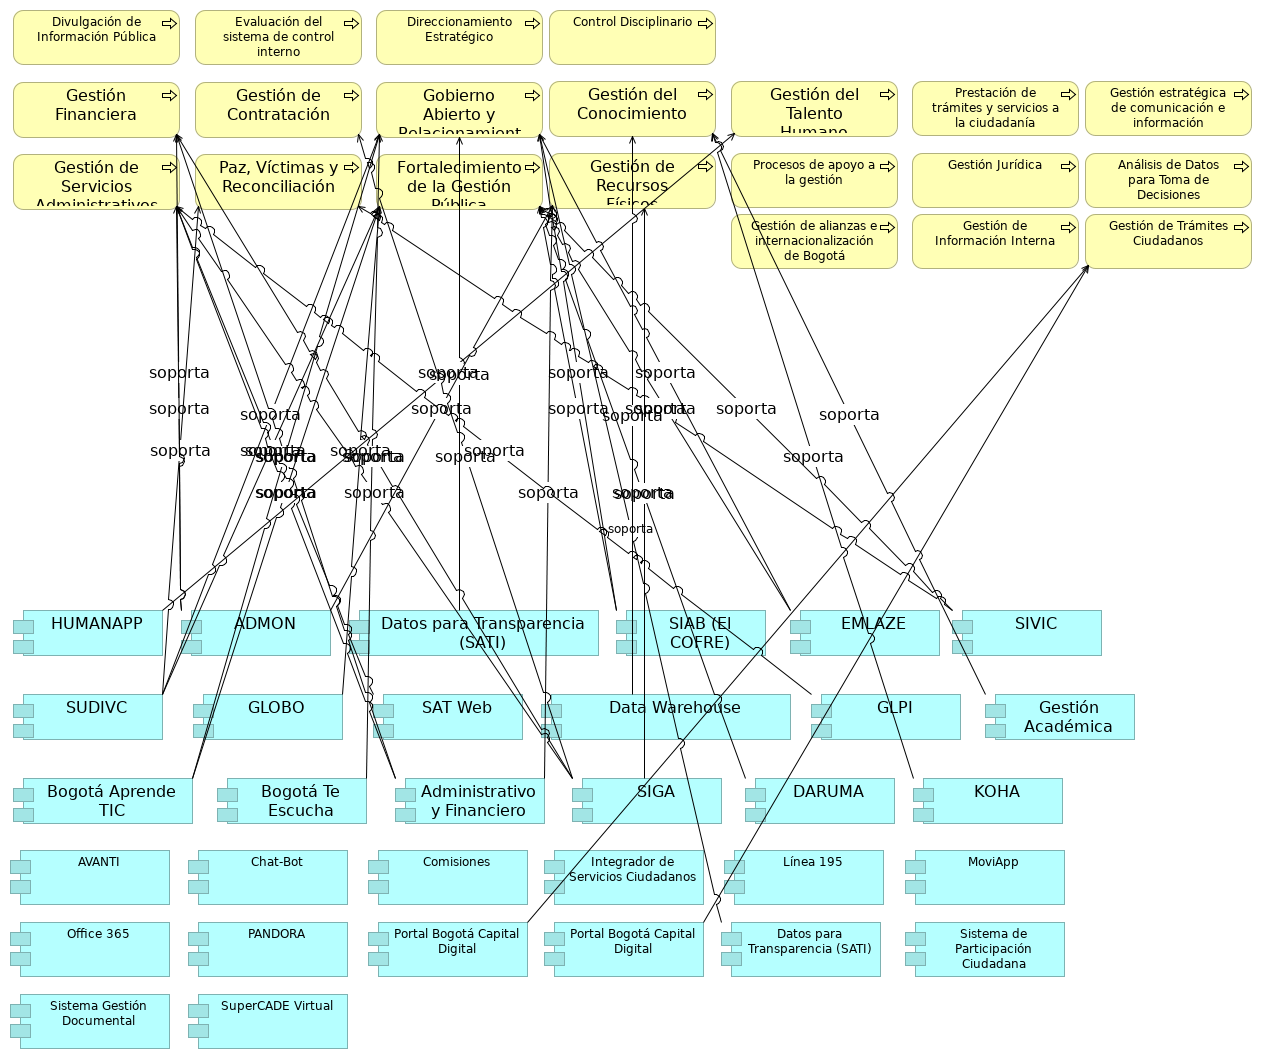
\includegraphics{images/06.2n3.a.AplicacionesyProcesos.png}
\caption{06.2n3.a.Aplicaciones y Procesos. \emph{Fuente: Propuesta
servicios de ingeniería y evaluación de arquitectura Arquitectura de
Aplicaciones Secretaria de la Alcaldía de Bogotá
(2025)}}\label{fig:id-7812cd6a3a0d4d5783b00f16f2c5826b}
\end{figure}

\subsubsection{Divulgación de Información
Pública}\label{sec:divulgaciuxf3n-de-informaciuxf3n-puxfablica}

Proceso de negocio para la difusión optimizada de información a través
de sistemas digitales.

\subsubsection{Evaluación del sistema de control
interno}\label{sec:evaluaciuxf3n-del-sistema-de-control-interno}

Evaluar de manera independiente y objetiva el Sistema de Control Interno
de la Secretaría General de la Alcaldía Mayor de Bogotá, mediante la
realización de auditorías internas de gestión, seguimientos e informes
regulatorios programados en el Plan de Anual de Auditorías, y la
atención a organismos de control, con el propósito de contribuir al
mejoramiento continuo de la gestión institucional.

\subsubsection{Direccionamiento
Estratégico}\label{sec:direccionamiento-estratuxe9gico}

Formular, implementar, hacer monitoreo y seguimiento a las políticas
públicas competencia de la Secretaría General, a los planes
institucionales, a los proyectos de inversión, y gestionar el
presupuesto de inversión mediante la definición de orientaciones,
metodologías, la retroalimentación, acompañamiento y articulación a las
dependencias de la entidad con el fin de cumplir el logro de la misión y
los objetivos institucionales, en el marco de una cultura de
transparencia.

\subsubsection{Control Disciplinario}\label{sec:control-disciplinario}

Adelantar los procesos disciplinarios contra los(as) servidores(as) y
exservidores(as) de la Secretaría General de la Alcaldía Mayor de Bogotá
D.C., y prevenir las conductas disciplinarias mediante la aplicación de
las normas vigentes en materia disciplinaria y el desarrollo de la
estrategia preventiva con el fin determinar la posible responsabilidad
disciplinaria, y evitar la ocurrencia de faltas disciplinarias por parte
de estos.

\subsubsection{Gestión del
Conocimiento}\label{sec:gestiuxf3n-del-conocimiento}

Gestionar el conocimiento y la innovación de la Secretaría General de la
Alcaldía Mayor de Bogotá, mediante la identificación, generación,
sistematización, análisis, transferencia y conservación del conocimiento
estratégico y la promoción de la innovación, con el fin de fortalecer el
aprendizaje, el mejoramiento organizacional y la toma de decisiones
basada en evidencias.

\subsubsection{Gestión del Talento
Humano}\label{sec:gestiuxf3n-del-talento-humano}

Gestionar el capital humano de la Secretaría General, y vincular y
administrar el Gabinete distrital y jefatura del talento humano interno
mediante el Plan Estratégico de Talento Humano para la Secretaría
General y el trámite de situaciones administrativas con el fin de
fortalecer el sentido de pertenencia y contribuir a la calidad de vida
del talento humano de la entidad.

\subsubsection{Prestación de trámites y servicios a la
ciudadanía}\label{sec:prestaciuxf3n-de-truxe1mites-y-servicios-a-la-ciudadanuxeda}

Proceso central para la interacción con los ciudadanos.

\subsubsection{Gestión estratégica de comunicación e
información}\label{sec:gestiuxf3n-estratuxe9gica-de-comunicaciuxf3n-e-informaciuxf3n}

Mantener informados a los distintos grupos de valor e interés acerca de
los programas, proyectos y gestión de la Administración Distrital a
través de la formulación y la implementación de estrategias de
comunicación pública con el propósito de interactuar y mantener la
confianza por parte de la entidad y de la ciudadanía en general.

\subsubsection{Gestión Financiera}\label{sec:gestiuxf3n-financiera}

Gestionar las operaciones financieras con cargo al presupuesto asignado
a la entidad, a través del registro de las operaciones económicas en
contabilidad para garantizar la elaboración y reporte de los estados
financieros a los entes de control en forma comprensible, relevante y
confiable, para que sean consultados por los ciudadanos y por los
interesados en la información financiera.

\subsubsection{Gestión de
Contratación}\label{sec:gestiuxf3n-de-contrataciuxf3n}

Gestionar la contratación de bienes, servicios y obras, mediante el
desarrollo de procesos contractuales transparentes y conforme a la
normativa legal vigente para satisfacer las necesidades de contratación
de las dependencias de la Secretaría General de la Alcaldía Mayor de
Bogotá, y contribuir al cumplimento de sus metas y objetivos.

\subsubsection{Gobierno Abierto y Relacionamiento con la
Ciudadanía}\label{sec:gobierno-abierto-y-relacionamiento-con-la-ciudadanuxeda}

Fortalecer relación entre la administración distrital y la ciudadanía
mediante la formulación de lineamientos, desarrollo de estrategias y
proyectos, fortalecimiento de capacidades, seguimiento y evaluación en
materia de servicio a la ciudadanía, gobierno abierto y transformación
digital de la Secretaría General y de las entidades distritales, para el
acceso oportuno, efectivo y de calidad a la oferta institucional de
bienes y servicios.

\subsubsection{Gestión de Recursos
Físicos}\label{sec:gestiuxf3n-de-recursos-fuxedsicos}

Administrar los bienes que legalmente están a cargo de la Secretaría
General de la Alcaldía Mayor de Bogotá D.C. mediante su recepción,
asignación, mantenimiento, control, baja y/o destinación final con el
fin de cubrir las necesidades de recursos físicos de las dependencias.

\subsubsection{Procesos de apoyo a la
gestión}\label{sec:procesos-de-apoyo-a-la-gestiuxf3n}

Procesos internos que facilitan la operación de la entidad.

\subsubsection{Gestión Jurídica}\label{sec:gestiuxf3n-juruxeddica}

Asesorar y representar jurídicamente a la Secretaría General de la
Alcaldía Mayor Bogotá D.C. mediante el análisis, trámite, defensa,
solución y respuesta de asuntos de carácter jurídico que surjan en el
desarrollo de las funciones de acuerdo con la normatividad vigente.

\subsubsection{Análisis de Datos para Toma de
Decisiones}\label{sec:anuxe1lisis-de-datos-para-toma-de-decisiones}

Proceso de negocio que utiliza software especializado para el análisis
de datos.

\subsubsection{Gestión de Servicios Administrativos y
Tecnológicos}\label{sec:gestiuxf3n-de-servicios-administrativos-y-tecnoluxf3gicos}

Apoyar la gestión de la Entidad a través de la prestación de los
servicios administrativos y tecnológicos, así como, de la gestión
documental, con el fin de satisfacer las necesidades de las dependencias
en la materia, al igual que conservar y preservar la memoria
institucional.

\subsubsection{Paz, Víctimas y
Reconciliación}\label{sec:paz-vuxedctimas-y-reconciliaciuxf3n}

Gestionar políticas, programas y estrategias dirigidas a las víctimas,
población en proceso de reintegración, reincorporación, comparecientes
de fuerza pública y ciudadanía en general por medio de la asistencia,
atención, reparación, y acciones de memoria, reconciliación y
construcción de paz territorial con el propósito de que Bogotá sea un
territorio de paz y reconciliación, donde todos puedan volver a empezar.

\subsubsection{Fortalecimiento de la Gestión
Pública}\label{sec:fortalecimiento-de-la-gestiuxf3n-puxfablica}

Generar capacidades institucionales en las entidades distritales a
través del desarrollo de estudios, investigaciones y estrategias
relacionadas con el fortalecimiento de la gestión, impresión de artes
gráficas y la publicación de la Gaceta Pública en el registro distrital;
con el fin, de modernizar y mejorar el desempeño de la administración
distrital.

\subsubsection{Gestión de alianzas e internacionalización de
Bogotá}\label{sec:gestiuxf3n-de-alianzas-e-internacionalizaciuxf3n-de-bogotuxe1}

Facilitar acciones estratégicas de cooperación, relacionamiento y
posicionamiento internacional, mediante la gestión de interacciones con
actores nacionales e internacionales, con el fin de movilizar recursos
técnicos y financieros, generar alianzas estratégicas y posicionar a
Bogotá como un referente global. De esta manera, se contribuirá a la
implementación del Plan de Desarrollo Distrital, fortalecerá las
políticas públicas y la gestión del Distrito, y se alineará con
iniciativas globales como la Agenda 2030.

\subsubsection{Gestión de Información
Interna}\label{sec:gestiuxf3n-de-informaciuxf3n-interna}

Proceso de recolección, procesamiento y distribución de información
dentro de la entidad.

\subsubsection{Gestión de Trámites
Ciudadanos}\label{sec:gestiuxf3n-de-truxe1mites-ciudadanos}

Proceso de atención y resolución de solicitudes y gestiones de los
ciudadanos.

\subsubsection{HUMANAPP}\label{sec:humanapp}

Apoya la gestión del talento humano.

\subsubsection{ADMON}\label{sec:admon}

Se relaciona con la gestión financiera, gestión de servicios
administrativos y tecnológicos, y gestión de recursos físicos.

\subsubsection{Datos para Transparencia
(SATI)}\label{sec:datos-para-transparencia-sati}

Plataforma que facilita el acceso público a datos e información
gubernamental. Soporta el proceso de Gobierno abierto y relacionamiento
con la ciudadanía.

\subsubsection{SIAB (El COFRE)}\label{sec:siab-el-cofre}

Sistema de Información del Archivo de Bogotá SIAB. Permite automatizar
los procesos archivísticos y técnicos que realiza el Archivo, tales como
llevar un registro de los Ingresos Documentales (antes área de acopio),
para la descripción y catalogación de la documentación, propios del
proceso de Gestión de la Función Archivística y del Patrimonio
Documental, para su custodia y conservación permanente. Utilizado en los
procesos de Gobierno abierto y relacionamiento con la ciudadanía, y
Fortalecimiento de la Gestión Pública.

\subsubsection{EMLAZE}\label{sec:emlaze}

Utilizado en los procesos de Gobierno abierto y relacionamiento con la
ciudadanía, y Fortalecimiento de la Gestión Pública.

\subsubsection{SIVIC}\label{sec:sivic}

Interviene en los procesos de Paz, víctimas y reconciliación, y
Fortalecimiento de la Gestión Pública.

\subsubsection{SUDIVC}\label{sec:sudivc}

Se aplica en los procesos de Gobierno abierto y relacionamiento con la
ciudadanía, Paz, víctimas y reconciliación, y Fortalecimiento de la
Gestión Pública.

\subsubsection{GLOBO}\label{sec:globo}

Utilizado en el proceso de Fortalecimiento de la Gestión Pública.

\subsubsection{SAT Web}\label{sec:sat-web}

Relacionado con la gestión de servicios administrativos y tecnológicos.

\subsubsection{Data Warehouse}\label{sec:data-warehouse}

Almacenes de datos de trabajo de SG.

\subsubsection{GLPI}\label{sec:glpi}

Soporta la gestión de servicios administrativos y tecnológicos.

\subsubsection{Gestión Académica}\label{sec:gestiuxf3n-acaduxe9mica}

Relacionado con la Gestión del conocimiento.

\subsubsection{Bogotá Aprende TIC}\label{sec:bogotuxe1-aprende-tic}

Apoya los procesos de Gobierno abierto y relacionamiento con la
ciudadanía, y Fortalecimiento de la Gestión Pública.

\subsubsection{Bogotá Te Escucha}\label{sec:bogotuxe1-te-escucha}

Es fundamental para el proceso de Gobierno abierto y relacionamiento con
la ciudadanía. También se menciona como el Sistema Distrital para la
Gestión de Peticiones Ciudadanas, a través del cual se evalúa la calidad
de las respuestas emitidas a la ciudadanía.

\subsubsection{Administrativo y
Financiero}\label{sec:administrativo-y-financiero}

Soporta la gestión financiera, gestión de servicios administrativos y
tecnológicos, y gestión de recursos físicos.

\subsubsection{SIGA}\label{sec:siga}

Interviene en la gestión de contratación, gestión financiera, gestión de
servicios administrativos y tecnológicos, y gestión de recursos físicos.

\subsubsection{DARUMA}\label{sec:daruma}

Se utiliza en el proceso de Fortalecimiento de la Gestión Pública.
También es el aplicativo donde se encuentran definidas las fichas
técnicas de productos y servicios de la Secretaría General y se
gestionan los riesgos estratégicos.

\subsubsection{KOHA}\label{sec:koha}

Relacionado con la Gestión del conocimiento.

\subsubsection{AVANTI}\label{sec:avanti}

Apoya la Gestión del conocimiento.

\subsubsection{Chat-Bot}\label{sec:chat-bot}

Canal web de atención a ciudadanía.

\subsubsection{Comisiones}\label{sec:comisiones}

Sesión levantamiento no. 1.

\subsubsection{Integrador de Servicios
Ciudadanos}\label{sec:integrador-de-servicios-ciudadanos}

Plataforma unificada para acceder a servicios y trámites ciudadanos.

\subsubsection{Línea 195}\label{sec:luxednea-195}

Canal telefónico de atención a ciudadanía.

\subsubsection{MoviApp}\label{sec:moviapp}

Canal movil de atención a ciudadanía. Sesión levantamiento no. 2.

\subsubsection{Office 365}\label{sec:office-365}

Ofimática y colaboración SG.

\subsubsection{PANDORA}\label{sec:pandora}

Implementación de temas precontractual y planeación.

\subsubsection{Portal Bogotá Capital
Digital}\label{sec:portal-bogotuxe1-capital-digital}

Plataforma de Trámites en línea. Portal Integrador de trámites y
servicios ofrecidos a la ciudadanía. Componente de aplicación que
permite la realización de trámites digitales.

\subsubsection{Portal Bogotá Capital
Digital}\label{sec:portal-bogotuxe1-capital-digital-1}

Plataforma de Trámites en línea. Portal Integrador de trámites y
servicios ofrecidos a la ciudadanía. Componente de aplicación que
permite la realización de trámites digitales.

\subsubsection{Datos para Transparencia
(SATI)}\label{sec:datos-para-transparencia-sati-1}

Plataforma que facilita el acceso público a datos e información
gubernamental. Soporta el proceso de Gobierno abierto y relacionamiento
con la ciudadanía.

\subsubsection{Sistema de Participación
Ciudadana}\label{sec:sistema-de-participaciuxf3n-ciudadana}

Componente de aplicación para facilitar la interacción y el acercamiento
(realimentación) de los ciudadanos.

\subsubsection{Sistema Gestión
Documental}\label{sec:sistema-gestiuxf3n-documental}

Componente de aplicación para la gestión electrónica de documentos.

\subsubsection{SuperCADE Virtual}\label{sec:supercade-virtual}

Red de canales presenciales de atención a
ciudadanía.\sidenote{This is a sidenote. This template features a large margin specifically so you can put notes, figures, tables and other things into it as additional material to the main content in the text block.}

Donec in elit ac ante vestibulum rhoncus. Pellentesque ligula tortor, aliquet malesuada nulla tristique vitae. Aliquam mi sem, varius eu pellentesque et, tristique nec quam. Vestibulum pellentesque in dui et venenatis. Sed malesuada elit pellentesque sapien aliquet porta. In at facilisis diam. Duis id ante tellus.\sidenote[][2cm]{This sidenote has been pushed down the page manually with an optional parameter, otherwise it would be right under the one above.} % This first optional argument to a sidenote is the symbol to use (leave this empty for automatic numbering) and the second is the vertical offset (positive is down, negative is up)

In diam libero, vulputate quis accumsan non, auctor in ipsum. Praesent cursus velit eget lacus sodales porta. Proin quis risus ut velit euismod scelerisque ut sed neque. Cras sagittis, dolor ac ullamcorper auctor, tortor dui facilisis diam, at sagittis nisi ipsum a neque. Nullam vel mattis nisi. Ut interdum ut diam at ornare. Nulla ultrices elit justo, vitae tristique massa vulputate sit amet.

\nonumsidenote{
	}Vestibulum erat felis, cursus vitae convallis ac, commodo eu nisi. Nulla facilisi. Mauris dignissim nisi felis, a mollis ex accumsan vel. Suspendisse bibendum vitae nibh in suscipit. Vestibulum et finibus eros. Nulla facilisi. Cras luctus aliquam finibus. In nec justo nec orci malesuada faucibus.

\subsubsection{Subsubsection Title} % Third level section

\begin{fullwidth} % Use the whole page width
	\textit{This is an example of a full width paragraph\ldots} Curabitur id placerat orci. Vivamus pulvinar augue ac feugiat blandit. Donec in ultricies mi. Nam eu lacus ac augue aliquet consectetur. Praesent dui risus, sollicitudin nec felis ut, posuere ultricies dolor. Sed massa nulla, dignissim eget sem sit amet, eleifend fermentum dui. Phasellus consequat sem vel turpis finibus, a aliquam risus malesuada.
\end{fullwidth}

Maecenas consectetur metus at tellus finibus condimentum. Proin arcu lectus, ultrices non tincidunt et, tincidunt ut quam. Integer luctus posuere est, non maximus ante dignissim quis. Nunc a cursus erat. Curabitur suscipit nibh in tincidunt sagittis. Nam malesuada vestibulum quam id gravida. Proin ut dapibus velit. Vestibulum eget quam quis ipsum semper convallis. Duis consectetur nibh ac diam dignissim, id condimentum enim dictum. Nam aliquet ligula eu magna pellentesque, nec sagittis leo lobortis. Aenean tincidunt dignissim egestas. Morbi efficitur risus ante, id tincidunt odio pulvinar vitae.

\paragraph{Paragraph Title} % Fourth level section

Lorem ipsum dolor sit amet, consectetur adipiscing elit. Aliquam auctor mi risus, quis tempor libero hendrerit at. Duis hendrerit placerat quam et semper. Nam ultricies metus vehicula arcu viverra, vel ullamcorper justo elementum. Pellentesque vel mi ac lectus cursus posuere et nec ex.

The section titles below show how multi-line section titles look at the 3 top levels.


%----------------------------------------------------------------------------------------
%	QUOTATIONS
%----------------------------------------------------------------------------------------

\section{Quotations}

Proin mollis urna posuere fringilla. Curabitur finibus, neque vitae vestibulum vestibulum, dolor sapien tincidunt augue, vel porta mauris metus nec mauris. Integer erat magna, porta id erat sed, lacinia volutpat erat. Nulla fermentum tellus arcu, eu iaculis ipsum malesuada aliquam. Duis et lacus maximus, consectetur metus et, eleifend arcu. Vestibulum condimentum diam vitae diam tincidunt viverra.\sidenotequote[-1cm]{\textbf{\LARGE ``}Lorem ipsum dolor sit amet, consectetur adipiscing elit. Praesent porttitor arcu luctus, imperdiet urna iaculis, mattis eros. Pellentesque iaculis odio vel nisl ullamcorper, nec faucibus ipsum molestie.\textbf{''}\\[4pt]\hfill--- John Smith, 1972} % Example margin quotation using the \sidenotequote custom command

\begin{quote}
	\textbf{\LARGE ``}Lorem ipsum dolor sit amet, consectetur adipiscing elit. Praesent porttitor arcu luctus, imperdiet urna iaculis, mattis eros. Pellentesque iaculis odio vel nisl ullamcorper, nec faucibus ipsum molestie. Sed dictum nisl non aliquet porttitor. Etiam vulputate arcu dignissim, finibus sem et, viverra nisl. Aenean luctus congue massa, ut laoreet metus ornare in.\textbf{''}
	
	\hfill--- John Smith, 1972
\end{quote}

Suspendisse tempus odio sit amet volutpat suscipit. Pellentesque ornare libero lacus, non fringilla dolor placerat in. Ut maximus ullamcorper lectus, a pharetra mi sagittis aliquet. Scelerisque augue sed mi fringilla, vel dapibus ligula finibus. Sed ornare velit sem, ac venenatis velit dignissim. Vestibulum ultrices mi at tincidunt condimentum.

%----------------------------------------------------------------------------------------
%	TABLES
%----------------------------------------------------------------------------------------

\section{Table Examples}

This statement automatically references the table below using its label: Table \ref{tab:example}.

%------------------------------------------------

\begin{margintable} % Use the margintable environment for tables to be output to the margin
	\footnotesize % Reduce the font size in the table as space is at a premium
	\caption{Margin table caption.}
	\begin{tabular}{L{0.22\linewidth} C{0.22\linewidth} R{0.25\linewidth}}
		\toprule
		\textbf{Year} & \textbf{Qtr.} & \textbf{Perf.}\\
		\midrule
		20XX & Q1 & 0.5\%\\
		20XX & Q2 & 26.5\%\\
		20XX & Q1 & 35.4\%\\
		20XX & Q4 & 41.3\%\\
		\bottomrule
	\end{tabular}
\end{margintable}

%------------------------------------------------

\begin{table}[H] % [H] forces the table to be output where it is defined in the code (it suppresses floating)
	\caption{Text block table caption.}
	\begin{tabular}{L{0.35\linewidth} L{0.38\linewidth} L{0.16\linewidth}}
		\toprule
		\textbf{Prospect} & \textbf{Industry} & \textbf{Revenue} \\
		\midrule
		Gerlach Inc & Business Development & 3M\\
		Doyle and Sons & Law & 1M\\
		Heathcote Group & Consulting & 12M\\
		Goyette Inc & Advertising & 5M\\
		Holzdeppe GmbH & Manufacturing & 23M\\
		Bienias AG & Accounting & 2.5M\\
		\bottomrule
	\end{tabular}
	\label{tab:example}
\end{table}

%------------------------------------------------

\begin{table*} % Use the table* environment for full width tables
	\caption{Full width table caption.}
	\begin{tabular}{C{0.03\linewidth} L{0.25\linewidth} L{0.27\linewidth} L{0.16\linewidth} L{0.16\linewidth}}
		\toprule
		\textit{\#} & \textbf{Prospect} & \textbf{Industry} & \textbf{Revenue} & \textbf{Employees} \\
		\midrule
		\textit{1} & Gerlach Inc & Business Development & 3M & 65\\
		\textit{2} & Doyle and Sons & Law & 1M & 15\\
		\textit{3} & Heathcote Group & Consulting & 12M & 250\\
		\textit{4} & Goyette Inc & Advertising & 5M & 100\\
		\textit{5} & Holzdeppe GmbH & Manufacturing & 23M & 75\\
		\textit{6} & Bienias AG & Accounting & 2.5M & 40\\
		\bottomrule
	\end{tabular}
\end{table*}

%----------------------------------------------------------------------
%	FIGURES
%----------------------------------------------------------------------

\section{Figure Examples}

This statement automatically references the figure below using its label: Figure \ref{fig:example}.

%------------------------------------------------

\begin{marginfigure} % Use the marginfigure environment for figures to be output to the margin
	
\includegraphics[width=\linewidth]{./include/placeholder.jpg}
	\caption{Margin figure caption.}
\end{marginfigure}

%------------------------------------------------

\begin{figure}[H] % [H] forces the figure to be output where it is defined in the code (it suppresses floating)
	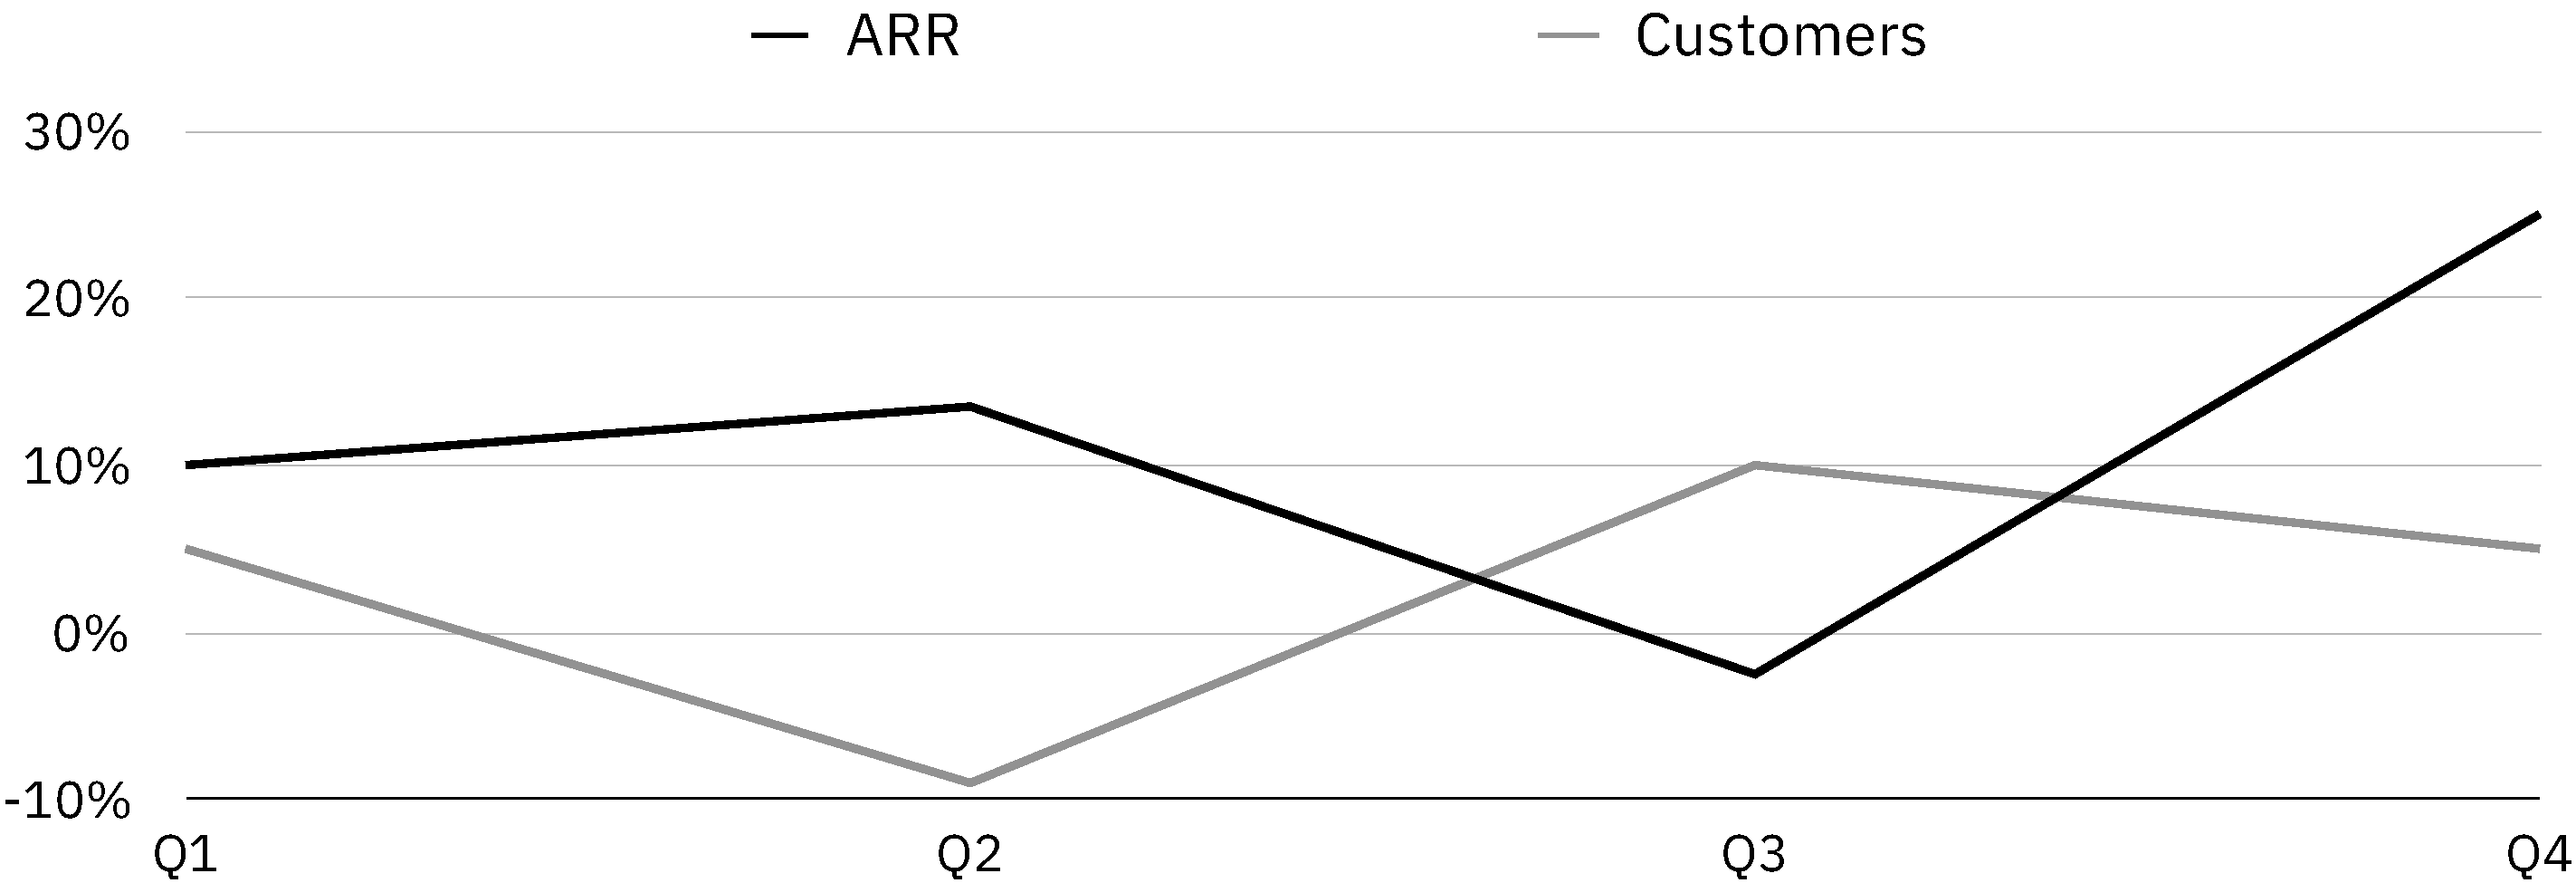
\includegraphics[width=\linewidth]{./include/ARR.pdf}
	\caption{Text block figure caption.}
	\label{fig:example} % Label for referencing this figure in the text automatically
\end{figure}

%------------------------------------------------

\begin{figure*} % Use the figure* environment for full width figures
	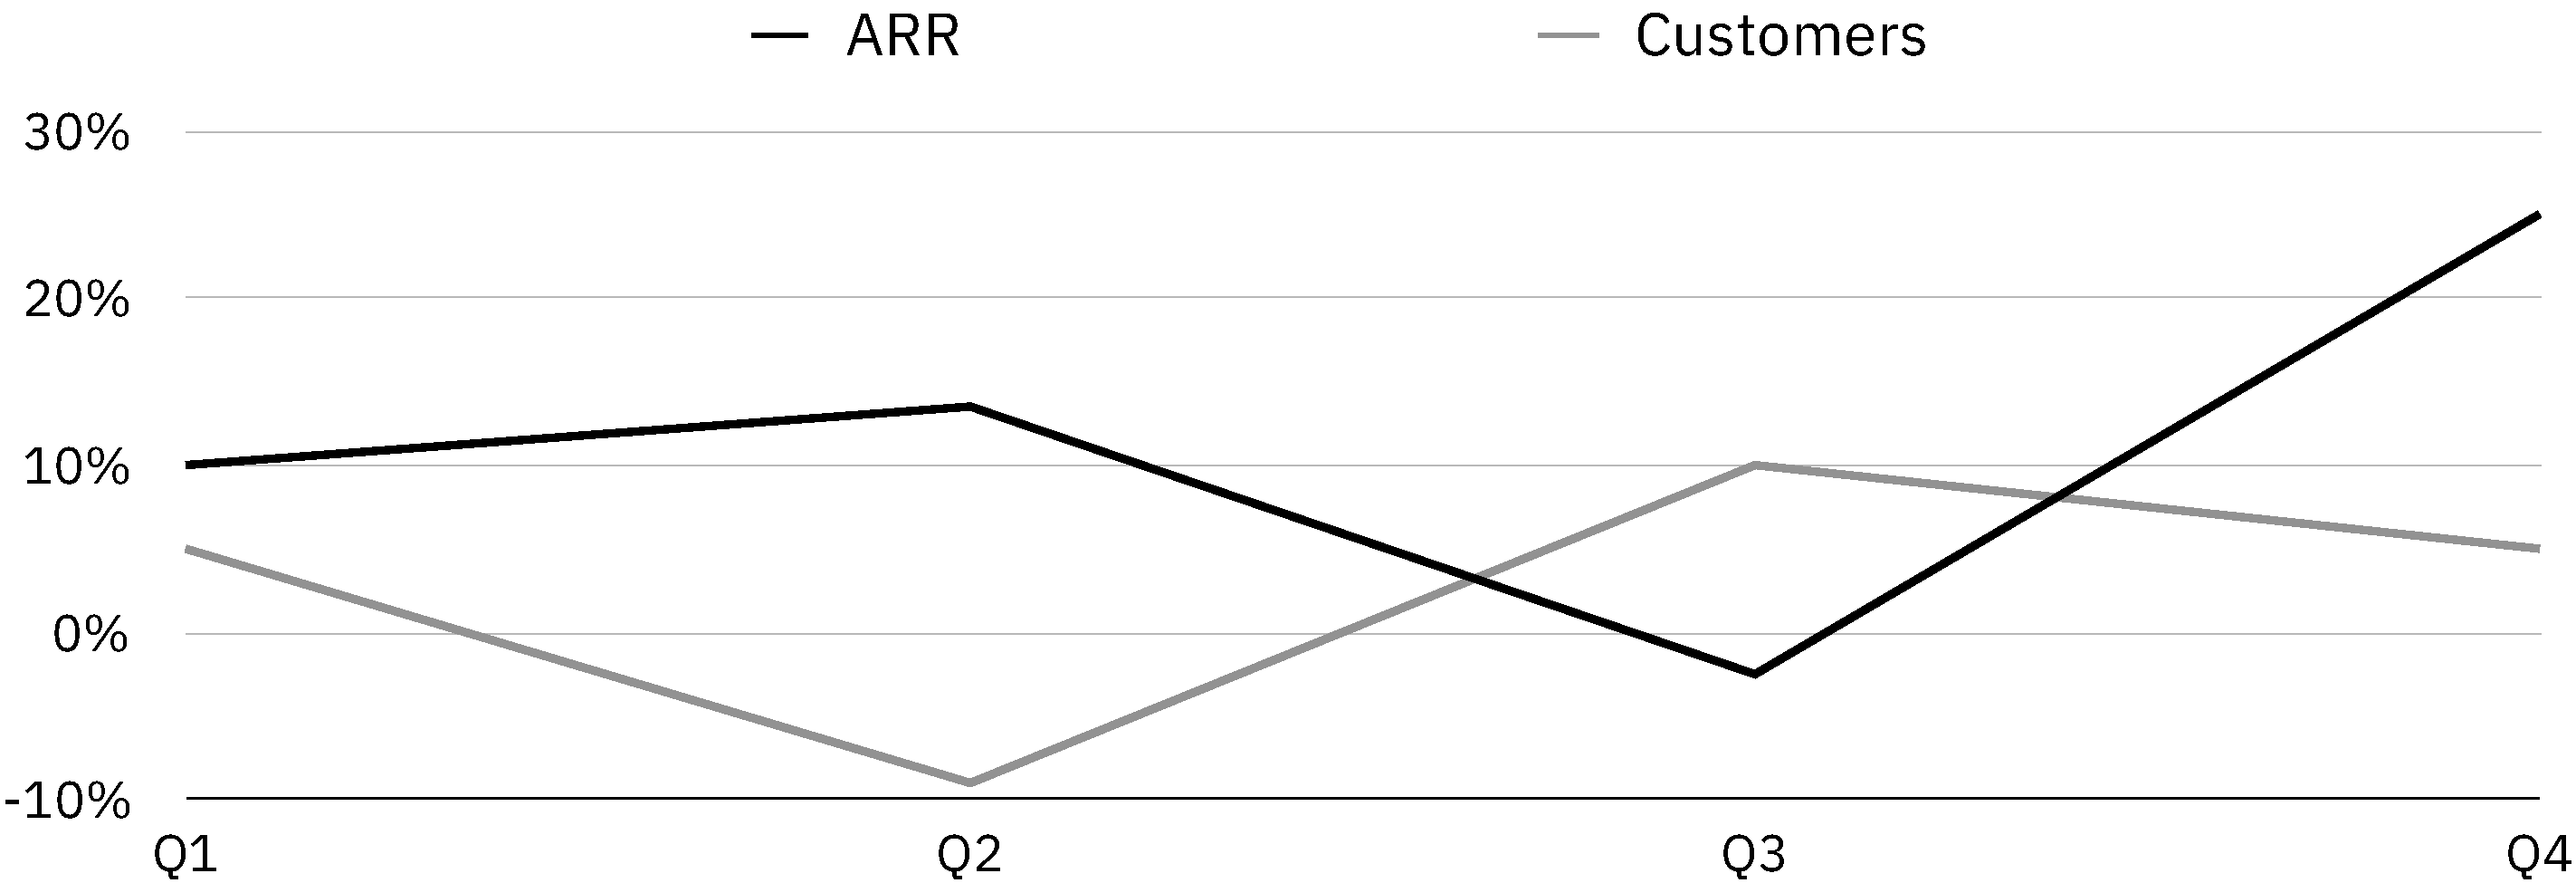
\includegraphics[width=\linewidth]{./include/ARR.pdf}
	\caption{Full width figure caption.}
\end{figure*}

%----------------------------------------------------------------------------------------
%	LISTS
%----------------------------------------------------------------------------------------

\section{List Examples}

\subsection{Bullet Point List}

\nonumsidenote{Bullet point lists can also be created in the margin. For these, we can remove the usual left margin to increase the available horizontal space:\\\medskip \begin{itemize}[leftmargin=*]\item Bullet item one. \item Bullet item two. \item Bullet item three.\end{itemize}}Lorem ipsum dolor sit amet, consectetur adipiscing elit. Praesent porttitor arcu luctus, imperdiet urna iaculis, mattis eros. Pellentesque iaculis odio vel nisl ullamcorper, nec faucibus ipsum molestie. Sed dictum nisl non aliquet porttitor.

\begin{itemize}
	\item First bullet point item
	\begin{itemize}
		\item First indented bullet point item
		\item Second indented bullet point item
		\begin{itemize}
			\item First second-level indented bullet point item
			\item Second second-level indented bullet point item
		\end{itemize}
		\item Third indented bullet point item
	\end{itemize}
	\item Second bullet point item
	\item Third bullet point item
\end{itemize}

Etiam vulputate arcu dignissim, finibus sem et, viverra nisl. Aenean luctus congue massa, ut laoreet metus ornare in. Nunc fermentum nisi imperdiet lectus tincidunt vestibulum at ac elit. Nulla mattis nisl eu malesuada suscipit.

%------------------------------------------------

\subsection{Numbered List}

\nonumsidenote[-2.5cm]{Numbered lists can also be created in the margin. For these, we can remove the usual left margin to increase the available horizontal space:\\\medskip \begin{enumerate}[leftmargin=*]\item Numbered item one. \item Numbered item two. \item Numbered item three.\end{enumerate}}Lorem ipsum dolor sit amet, consectetur adipiscing elit. Praesent porttitor arcu luctus, imperdiet urna iaculis, mattis eros. Pellentesque iaculis odio vel nisl ullamcorper, nec faucibus ipsum molestie. Sed dictum nisl non aliquet porttitor.

\begin{enumerate}
	\item First numbered item
	\begin{enumerate}
		\item First indented numbered item
		\item Second indented numbered item
		\begin{enumerate}
			\item First second-level indented numbered item
			\item Second second-level indented numbered item
		\end{enumerate}
		\item Third indented numbered item
	\end{enumerate}
	\item Second numbered item
	\item Third numbered item
\end{enumerate}

Etiam vulputate arcu dignissim, finibus sem et, viverra nisl. Aenean luctus congue massa, ut laoreet metus ornare in. Nunc fermentum nisi imperdiet lectus tincidunt vestibulum at ac elit. Nulla mattis nisl eu malesuada suscipit.

%------------------------------------------------

\subsection{Description List}

\nonumsidenote{Description lists can also be created in the margin:\\\medskip \begin{description}\item[A1] Description item one. \item[B1] Description item two. \item[C1] Description item three.\end{description}}Lorem ipsum dolor sit amet, consectetur adipiscing elit. Praesent porttitor arcu luctus, imperdiet urna iaculis, mattis eros. Pellentesque iaculis odio vel nisl ullamcorper, nec faucibus ipsum molestie. Sed dictum nisl non aliquet porttitor.

\begin{description}
	\item[Item One] Lorem ipsum dolor sit amet, consectetur adipiscing elit. Praesent porttitor arcu luctus, imperdiet urna iaculis, mattis eros. Pellentesque iaculis odio vel nisl ullamcorper, nec faucibus ipsum molestie.
	\item[Item Two] Sed dictum nisl non aliquet porttitor.
	\begin{description}
		\item[Subitem] Maecenas consectetur metus at tellus finibus condimentum. Proin arcu lectus, ultrices non tincidunt et, tincidunt ut quam. Integer luctus posuere est, non maximus ante dignissim quis.
		\begin{description}
			\item[Subsubitem] Maecenas consectetur metus at tellus finibus condimentum. Proin arcu lectus, ultrices non tincidunt et, tincidunt ut quam. Integer luctus posuere est, non maximus ante dignissim quis.
	\end{description}
	\end{description}
	\item[Item Three] Etiam vulputate arcu dignissim, finibus sem et, viverra nisl. Aenean luctus congue massa, ut laoreet metus ornare in. Nunc fermentum nisi imperdiet lectus tincidunt vestibulum at ac elit. Nulla mattis nisl eu malesuada suscipit.
\end{description}

Etiam vulputate arcu dignissim, finibus sem et, viverra nisl. Aenean luctus congue massa, ut laoreet metus ornare in.

%----------------------------------------------------------------------------------------
%	REFERENCING CITATIONS
%----------------------------------------------------------------------------------------

\section{Referencing Citations}

This statement requires citation \autocite{Smith:2024jd}.

This statement requires multiple citations \autocite{Smith:2024jd, Smith:2023qr}.

This short citation is in the margin\sidecite{Smith:2023qr}.

This long citation is in the margin\fullsidecite{Smith:2024jd}.

This statement has an in-text citation: \textcite{Smith:2024jd}.

%----------------------------------------------------------------------------------------
%	LINKS
%----------------------------------------------------------------------------------------

\section{Link Examples}

This is a URL link: \href{https://www.duckduckgo.com}{DuckDuckGo}.\nonumsidenote{Links can be clicked in the PDF to navigate to the linked website or email address.}

This is a email link: \href{mailto:example@example.com}{example@example.com}.

This is a monospaced URL link: \url{https://duckduckgo.com}.


%----------------------------------------------------------------------------------------
%	CODE
%----------------------------------------------------------------------------------------

\section{Displaying Code}

The block below is a code listing. It displays code in an easy to use way with line numbers for quick reference to specific parts of the code.

\begin{lstlisting}
{
	"city": [
		{
			"id": 1,
			"name": "Toronto",
			"country": "Canada",
			"population": 6200000
		},
		{
			"id": 2,
			"name": "New York",
			"country": "United States of America",
			"population": 8800000
		}
	]
}
\end{lstlisting}

%----------------------------------------------------------------------------------------
%	 REFERENCES/BIBLIOGRAPHY
%----------------------------------------------------------------------------------------

\newpage

\addcontentsline{toc}{section}{Reference List} % Add the bibliography to the table of contents

\begin{twothirdswidth} % Content in this environment to be at two-thirds of the whole page width
	\printbibliography[title=Reference List] % Output the bibliography with a custom section title
\end{twothirdswidth}

%----------------------------------------------------------------------------------------
%	APPENDICES
%----------------------------------------------------------------------------------------

\newpage

\section*{Appendices}

\begin{appendices}

\section{Appendix Section}

Lorem ipsum dolor sit amet, consectetur adipiscing elit. Aliquam auctor mi risus, quis tempor libero hendrerit at. Duis hendrerit placerat quam et semper. Nam ultricies metus vehicula arcu viverra, vel ullamcorper justo elementum. Pellentesque vel mi ac lectus cursus posuere et nec ex. Fusce quis mauris egestas lacus commodo venenatis. Ut at arcu lectus. Donec et urna nunc. Morbi eu nisl cursus sapien eleifend tincidunt quis quis est. Donec ut orci ex. Praesent ligula enim, ullamcorper non lorem a, ultrices volutpat dolor. Nullam at imperdiet urna. Pellentesque nec velit eget euismod pretium.

\section{Appendix Section}

Lorem ipsum dolor sit amet, consectetur adipiscing elit. Aliquam auctor mi risus, quis tempor libero hendrerit at. Duis hendrerit placerat quam et semper. Nam ultricies metus vehicula arcu viverra, vel ullamcorper justo elementum. Pellentesque vel mi ac lectus cursus posuere et nec ex. Fusce quis mauris egestas lacus commodo venenatis. Ut at arcu lectus. Donec et urna nunc. Morbi eu nisl cursus sapien eleifend tincidunt quis quis est. Donec ut orci ex. Praesent ligula enim, ullamcorper non lorem a, ultrices volutpat dolor. Nullam at imperdiet urna. Pellentesque nec velit eget euismod pretium.

\section{Appendix Section}

Lorem ipsum dolor sit amet, consectetur adipiscing elit. Aliquam auctor mi risus, quis tempor libero hendrerit at. Duis hendrerit placerat quam et semper. Nam ultricies metus vehicula arcu viverra, vel ullamcorper justo elementum. Pellentesque vel mi ac lectus cursus posuere et nec ex. Fusce quis mauris egestas lacus commodo venenatis. Ut at arcu lectus. Donec et urna nunc. Morbi eu nisl cursus sapien eleifend tincidunt quis quis est. Donec ut orci ex. Praesent ligula enim, ullamcorper non lorem a, ultrices volutpat dolor. Nullam at imperdiet urna. Pellentesque nec velit eget euismod pretium.

\end{appendices}

%----------------------------------------------------------------------------------------

\end{document}
